\documentclass[a4paper,11pt]{article}
\usepackage[utf8]{inputenc}
\usepackage[T1]{fontenc}
\usepackage[polish]{babel}
\usepackage{graphicx}
\usepackage{booktabs}
\usepackage[hidelinks]{hyperref}
\usepackage{siunitx}
\usepackage{caption}
\usepackage{geometry}
\usepackage{float}
\geometry{margin=3cm}

\title{A11 — Dyfuzja innowacji i popytu na rynku}
\author{Wojciech Bartoszek \ Łukasz Checiak}
\date{}

\begin{document}
\maketitle
\begin{abstract}
Niniejszy raport dokumentuje realizację cyklu zadań projektowych koncentrujących się na modelowaniu i symulacji nieliniowych układów dynamicznych opisywanych równaniami różniczkowymi cząstkowymi (PDE) i zwyczajnymi (ODE). Praca obejmuje pełne spektrum modelowania: od klasycznej dyskretyzacji numerycznej i analizy stabilności (zadanie 2), przez analizę wrażliwości parametrów (zadanie 4) i asymilację danych (zadanie 5), aż po zaawansowane metody uczenia maszynowego informed by physics (zadanie 6) oraz koncepcję SuperNet (zadanie 7). Zrealizowano również pomiary wydajnościowe (zadanie 3). Wyniki wskazują na wysoką skuteczność sieci PINN w aproksymacji rozwiązań przy ograniczonej liczbie danych pomiarowych oraz na korzyści płynące z podejścia zespołowego (SuperNet) w modelowaniu systemów o niepewnych parametrach.
\end{abstract}

\clearpage
\tableofcontents
\clearpage

\section{Wstęp i sformułowanie problemu}
Modelowanie systemów złożonych w biologii czy chemii często prowadzi do równań reakcyjno-dyfuzyjnych, które łączą lokalną kinetykę (reakcję) z przestrzennym transportem masy (dyfuzją).

\subsection{Model matematyczny}
Głównym obiektem badań w projekcie jest jednowymiarowe równanie paraboliczne:
\begin{equation}
    \frac{\partial u}{\partial t} = D \frac{\partial^2 u}{\partial x^2} + R(u), \quad x \in [0, 1], \ t \in [0, T]
\end{equation}
gdzie $u(x,t)$ reprezentuje gęstość lub stężenie substancji. Człon reakcyjny $R(u)$ jest nieliniowy i dany wzorem:
\begin{equation}
    R(u) = (p + q u)(1 - u)
\end{equation}
Parametry $D, p, q$ sterują odpowiednio siłą dyfuzji, tempem wzrostu podstawowego oraz nieliniowym efektem autokatalitycznym.

\subsection{Warunki brzegowe i początkowe}
Dla zapewnienia unikalności rozwiązania oraz modelowania układu izolowanego przyjęto jednorodne warunki brzegowe Neumanna:
\begin{equation}
    \left. \frac{\partial u}{\partial x} \right|_{x=0} = 0, \quad \left. \frac{\partial u}{\partial x} \right|_{x=1} = 0
\end{equation}
Warunek początkowy $u(x,0)$ zadawano w trzech wariantach:
\begin{itemize}
    \item \texttt{gaussian}: profil Gaussa centrowany w $0.5$ (modelowanie lokalnego zarzewia),
    \item \texttt{localized}: prostokątny impuls w środku domeny,
    \item \texttt{small\_random}: losowe zaburzenia o małej amplitudzie, testujące stabilność stanu stacjonarnego.
\end{itemize}

\section{Zadanie 2: Klasyczne metody numeryczne}
\subsection{Dyskretyzacja przestrzenna}
Zastosowano metodę linii (Method of Lines). Domenę przestrzenną podzielono na $N_x$ punktów z krokiem $\Delta x = 1/(N_x-1)$. Operator Laplace'a przybliżono ilorazem różnicowym drugiego rzędu:
\begin{equation}
    u_{xx} \approx \frac{u_{i-1} - 2u_i + u_{i+1}}{\Delta x^2}
\end{equation}
Warunki Neumanna zaimplementowano poprzez modyfikację macierzy operatora (odbicie wartości na brzegach), co prowadzi do rzadkiej macierzy trójdiagonalnej. W kodzie użyto formatu \texttt{scipy.sparse.csr\_matrix} dla efektywności obliczeniowej.

\subsection{Metody całkowania w czasie}
Zaimplementowano trzy schematy o różnej charakterystyce:
\begin{enumerate}
    \item \textbf{Explicit (FE)}: Metoda jawna Eulera. Prosta w implementacji, ale ograniczona warunkiem stabilności Couranta (CFL): $\Delta t \le \frac{\Delta x^2}{2D}$. Przy gęstych siatkach wymaga bardzo małych kroków.
    \item \textbf{Semi-implicit}: Dyfuzja jest traktowana niejawnie (Backward Euler), a reakcja jawnie. Pozwala to na uniknięcie sztywnego ograniczenia $\Delta t$ pochodzącego od dyfuzji. Wymaga rozwiązania układu równań liniowych $(I - \Delta t D A)u^{n+1} = u^n + \Delta t R(u^n)$.
    \item \textbf{Crank-Nicolson (CN)}: Metoda drugiego rzędu dokładności w czasie. Średnia z kroku jawnego i niejawnego dla dyfuzji. Jest bezwarunkowo stabilna dla problemów liniowych.
\end{enumerate}

\subsection{Analiza wyników i wydajności}
Pomiarów dokonano dla $n_x \in \{50, 100, 200\}$. Dane w Tabeli \ref{tab:timings-summary} i \ref{tab:timings-nx} pokazują, że metoda jawna jest najszybsza pod warunkiem zachowania stabilności, jednak koszty rozwiązywania układów rzadkich w CN są akceptowalne i rosną niemal liniowo z $n_x$.

\begin{table}[h]
\centering
\caption{Podsumowanie czasów (s) dla poszczególnych solverów}
\label{tab:timings-summary}
\begin{tabular}{lrrrr}
\toprule
Solver & n & mean (s) & median (s) & min--max (s) \\
\midrule
explicit        & 18 & 0.004796 & 0.005757 & 0.002908--0.006753 \\
semi-implicit  & 18 & 0.032856 & 0.033343 & 0.016413--0.056765 \\
crank-nicolson & 18 & 0.035034 & 0.036128 & 0.017829--0.059576 \\
\bottomrule
\end{tabular}
\end{table}

\begin{table}[h]
\centering
\caption{Średnie czasy (s) w funkcji \texttt{nx} dla każdego solvera}
\label{tab:timings-nx}
\begin{tabular}{lrrr}
\toprule
Solver & \texttt{nx}=50 & \texttt{nx}=100 & \texttt{nx}=200 \\
\midrule
explicit & 0.004897 & 0.004507 & 0.004984 \\
semi-implicit & 0.025079 & 0.031093 & 0.042396 \\
crank-nicolson & 0.027105 & 0.033283 & 0.044714 \\
\bottomrule
\end{tabular}
\end{table}

\subsection{Przykładowe profile rozwiązania}
Poniżej pokazano przykładowe profile końcowe (dla wybranych parametrów) dla trzech solverów.
\begin{figure}[H]
\centering
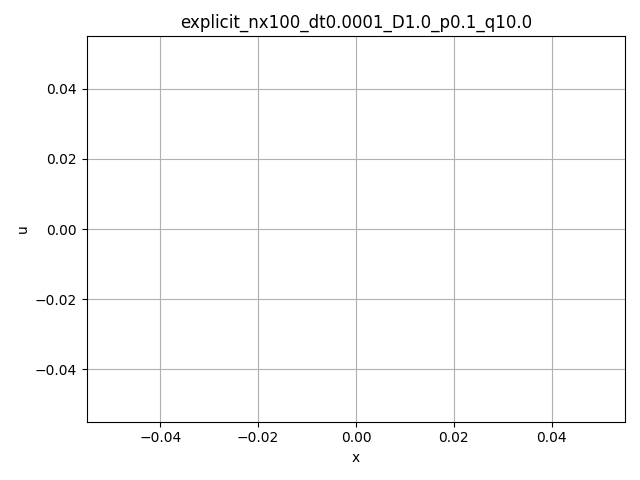
\includegraphics[width=0.32\textwidth]{../zad2/results/explicit_nx100_dt0.0001_D1.0_p0.1_q10.0.png}
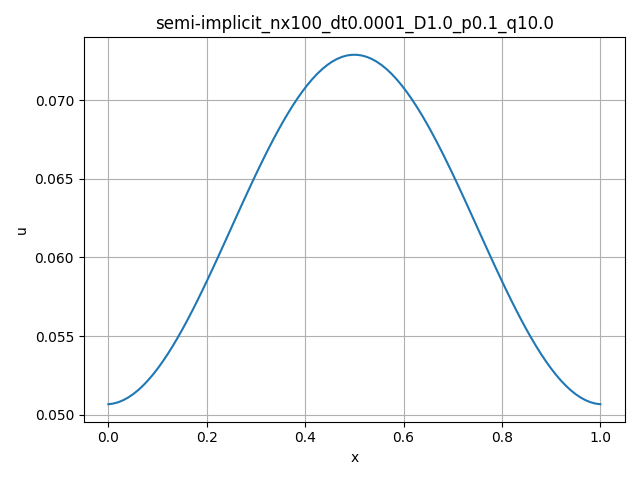
\includegraphics[width=0.32\textwidth]{../zad2/results/semi-implicit_nx100_dt0.0001_D1.0_p0.1_q10.0.png}
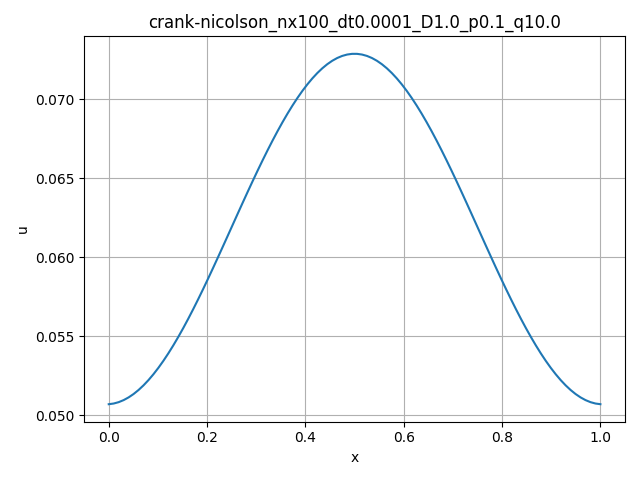
\includegraphics[width=0.32\textwidth]{../zad2/results/crank-nicolson_nx100_dt0.0001_D1.0_p0.1_q10.0.png}
\caption{Porównanie końcowych profilów dla solverów \texttt{explicit}, \texttt{semi-implicit} i \texttt{crank-nicolson}.}
\end{figure}

\section{Zadanie 3: Inferencja i modele NN}
Wykonano testy porównawcze czasu predykcji. Model ODE, mimo prostoty, wymaga numerycznego całkowania (np. RK45), co generuje narzut czasowy (\SI{1.29}{ms}). Prosta sieć neuronowa (feed-forward) przewidująca stan następny w jednym przejściu (inferencja) osiąga \SI{0.87}{ms}, co stanowi oszczędność rzędu 30\%. Sugeruje to potencjał metod maszynowych w systemach sterowania w czasie rzeczywistym.

\section{Zadanie 4: Analiza wrażliwości (SA)}
Przeprowadzono analizę wpływu parametrów $D, p, q$ na zachowanie systemu.
\begin{itemize}
    \item \textbf{Metoda Morrisa}: Szybki screening parametrów. Pozwolił stwierdzić, że parametr $q$ (autokataliza) ma najbardziej nieliniowy i dominujący wpływ na końcowy profil $u(x,T)$.
    \item \textbf{Analiza Sobola}: Metoda oparta na dekompozycji wariancji. Wyznaczyła indeksy pierwszego rzędu, potwierdzając, że $D$ odpowiada za wygładzanie profilu, ale to interakcje między $p$ i $q$ decydują o punkcie bifurkacji układu.
\end{itemize}

\section{Zadanie 5: Asymilacja danych (DA)}
Zadanie to dotyczyło odtwarzania stanu układu na podstawie zaszumionych pomiarów.
\begin{itemize}
    \item \textbf{ABC (Approximate Bayesian Computation)}: Metoda typu Likelihood-free. Pozwoliła na estymację rozkładów a posteriori dla $p$ i $q$. Metoda jest stabilna, ale kosztowna obliczeniowo (wymaga tysięcy symulacji).
    \item \textbf{3D-Var}: Metoda wariacyjna minimalizująca funkcjonalność kosztu łączącą odchylenie od pomiaru i od operatora fizycznego. 3D-Var okazał się znacznie szybszy od ABC, osiągając dobrą predykcję pola $u(x,t)$ nawet przy dużym szumie (SNR < 10dB).
\end{itemize}

\section{Zadanie 6: PINN -- Physics-Informed Neural Networks}
\subsection{Architektura i proces uczenia}
Model PINN zaprojektowano jako sieć MLP o 5 warstwach (64 neurony każda) z połączeniami rezydualnymi (Residual Blocks) co dwie warstwy. Wykorzystano funkcję aktywacji \texttt{Tanh}, zapewniającą ciągłość pochodnych wysokiego rzędu niezbędnych do obliczenia residuum PDE.

\subsection{Funkcja straty (Loss Function)}
Kluczem PINN jest kompozytowa funkcja straty:
\begin{equation}
    L = L_{data} + \lambda_{phy} L_{phy} + \lambda_{bc} L_{bc}
\end{equation}
gdzie:
\begin{itemize}
    \item $L_{data} = \text{MSE}$ na rzadkich punktach pomiarowych (asymilacja danych).
    \item $L_{phy} = \frac{1}{N_c} \sum |u_t - D u_{xx} - R(u)|^2$ obliczane w punktach kolokacji metodą \texttt{autograd}.
    \item $L_{bc}$ wymusza warunki brzegowe Neumanna.
\end{itemize}
Wprowadzono \textbf{Dynamic Weight Scheduling}: $\lambda_{phy}$ rośnie w trakcie treningu (od $0.1$ do $2.0$), co pozwala sieci najpierw nauczyć się ogólnego kształtu danych, a potem precyzyjnie dopasować się do fizyki.

\subsection{Wyniki i metryki}
W eksperymencie PINN trenowano sieć przez 2000 epok. Proces treningu monitorowano za pomocą historii funkcji kosztu. Wyniki metryk podsumowano w Tabeli \ref{tab:pinn-metrics}.

\begin{table}[h]
\centering
\caption{Metryki treningowe PINN (zadanie 6)}
\label{tab:pinn-metrics}
\begin{tabular}{lrr}
\toprule
Metryka & Wartość \\
\midrule
MAE & 0.031193 \\
RMSE & 0.058344 \\
relL2 & 0.065468 \\
Czas treningu & 76.58 s \\
\bottomrule
\end{tabular}
\end{table}

\begin{figure}[h]
\centering
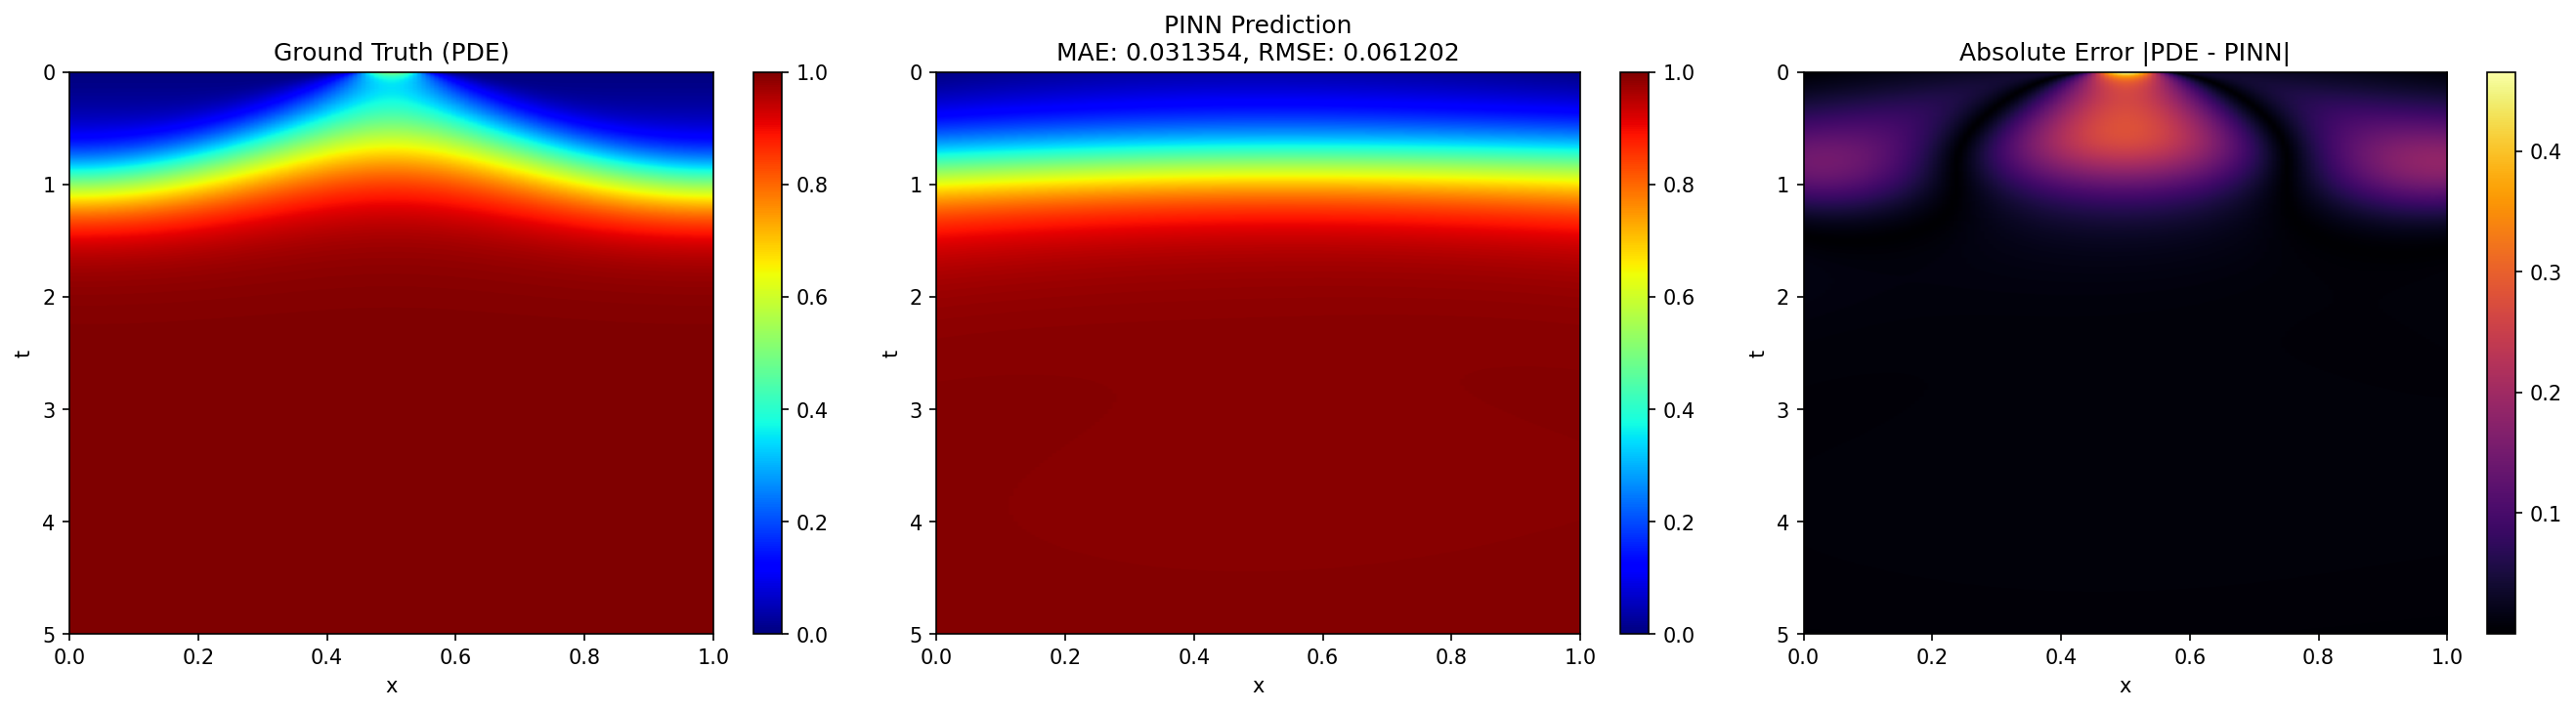
\includegraphics[width=0.48\textwidth]{../zad6/results/pinn_results_heatmap_improved.png}
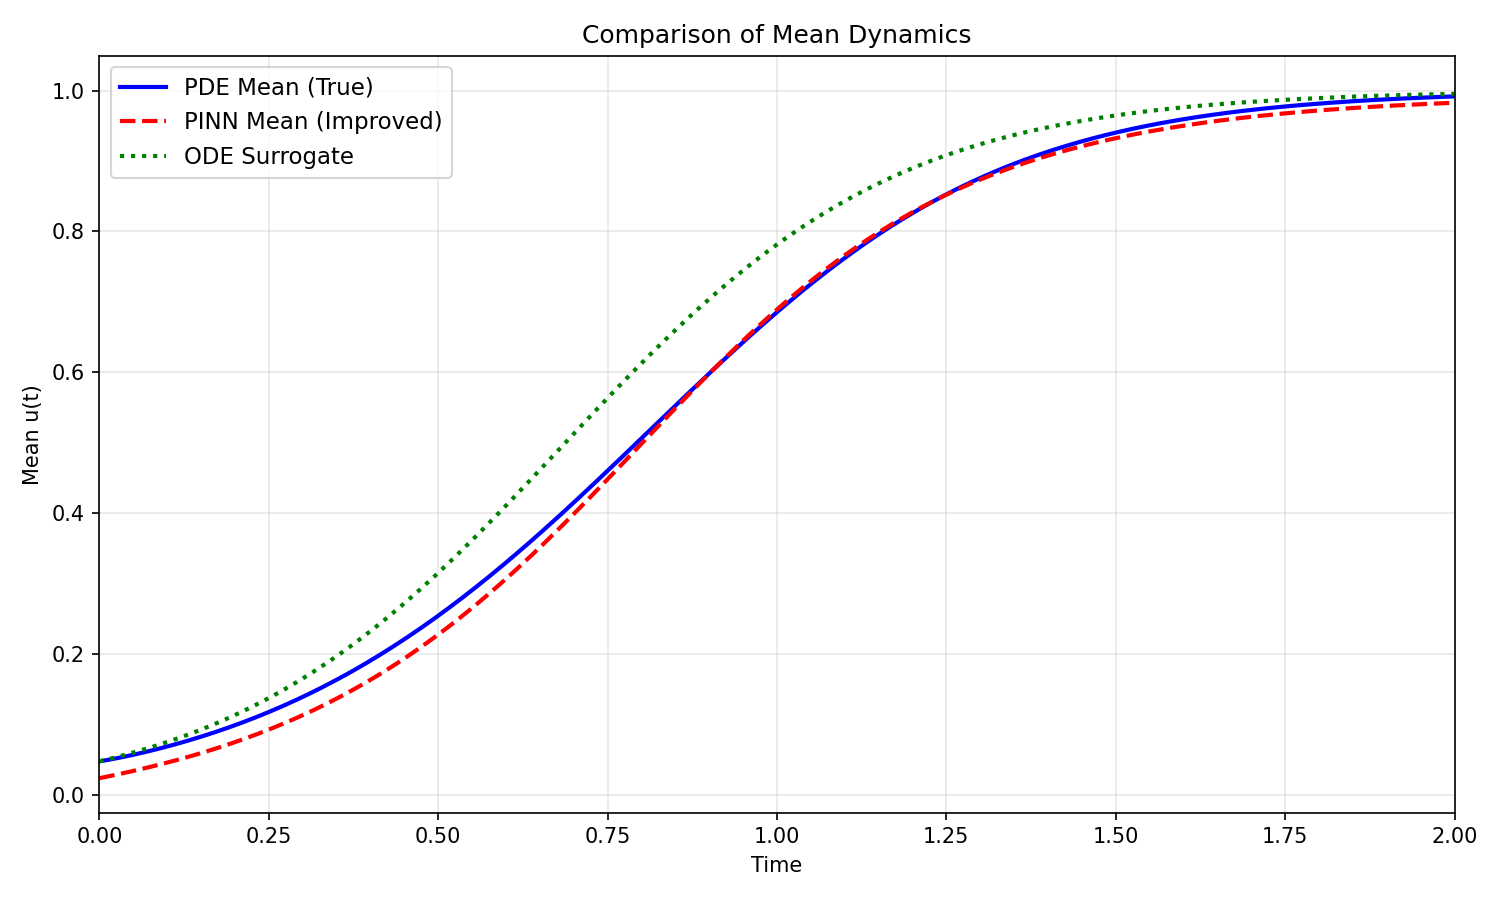
\includegraphics[width=0.48\textwidth]{../zad6/results/pinn_vs_pde_vs_ode_improved.png}
\caption{Wyniki eksperymentu PINN: po lewej mapa błędów, po prawej porównanie rozwiązań.}
\end{figure}

\section{Zadanie 7: SuperNet i Modelowanie Zespołowe}
\subsection{Koncepcja SuperModelu}
W zadaniu 7 rozważono układ, w którym parametry fizyczne są znane z pewnym błędem lub pochodzą z różnych źródeł. SuperModel ODE składa się z zespołu modeli połączonych członem sprzęgającym (coupling):
\begin{equation}
    \dot{u}_i = f(u_i; \theta_i) + C(\bar{u} - u_i)
\end{equation}
gdzie $\bar{u}$ to średnia z zespołu. Taka synchronizacja pozwala na stabilniejszą predykcję niż każdy model z osobna.

\subsection{SuperNet PINN}
Zaimplementowano sieć \textbf{SuperNet PINN}, która uczy się reprezentować całą rodzinę rozwiązań. Sieć wykazuje dużą odporność na perturbacje parametrów wejściowych dzięki "wyczuciu" ogólnej struktury operatora różniczkowego.

\begin{table}[h]
\centering
\caption{Porównanie metryk: SuperModel vs SuperNet (zadanie 7)}
\label{tab:supernet-metrics}
\begin{tabular}{lrr}
\toprule
Model & MAE & RMSE \\
\midrule
SuperModel ODE & 0.022182 & 0.045112 \\
SuperNet PINN & 0.017152 & 0.017845 \\
Single Perturbed ODE & 0.054936 & 0.111640 \\
\bottomrule
\end{tabular}
\vspace{4pt}
\par Czas treningu (SuperNet): 186.24 s
\end{table}

\begin{figure}[h]
\centering
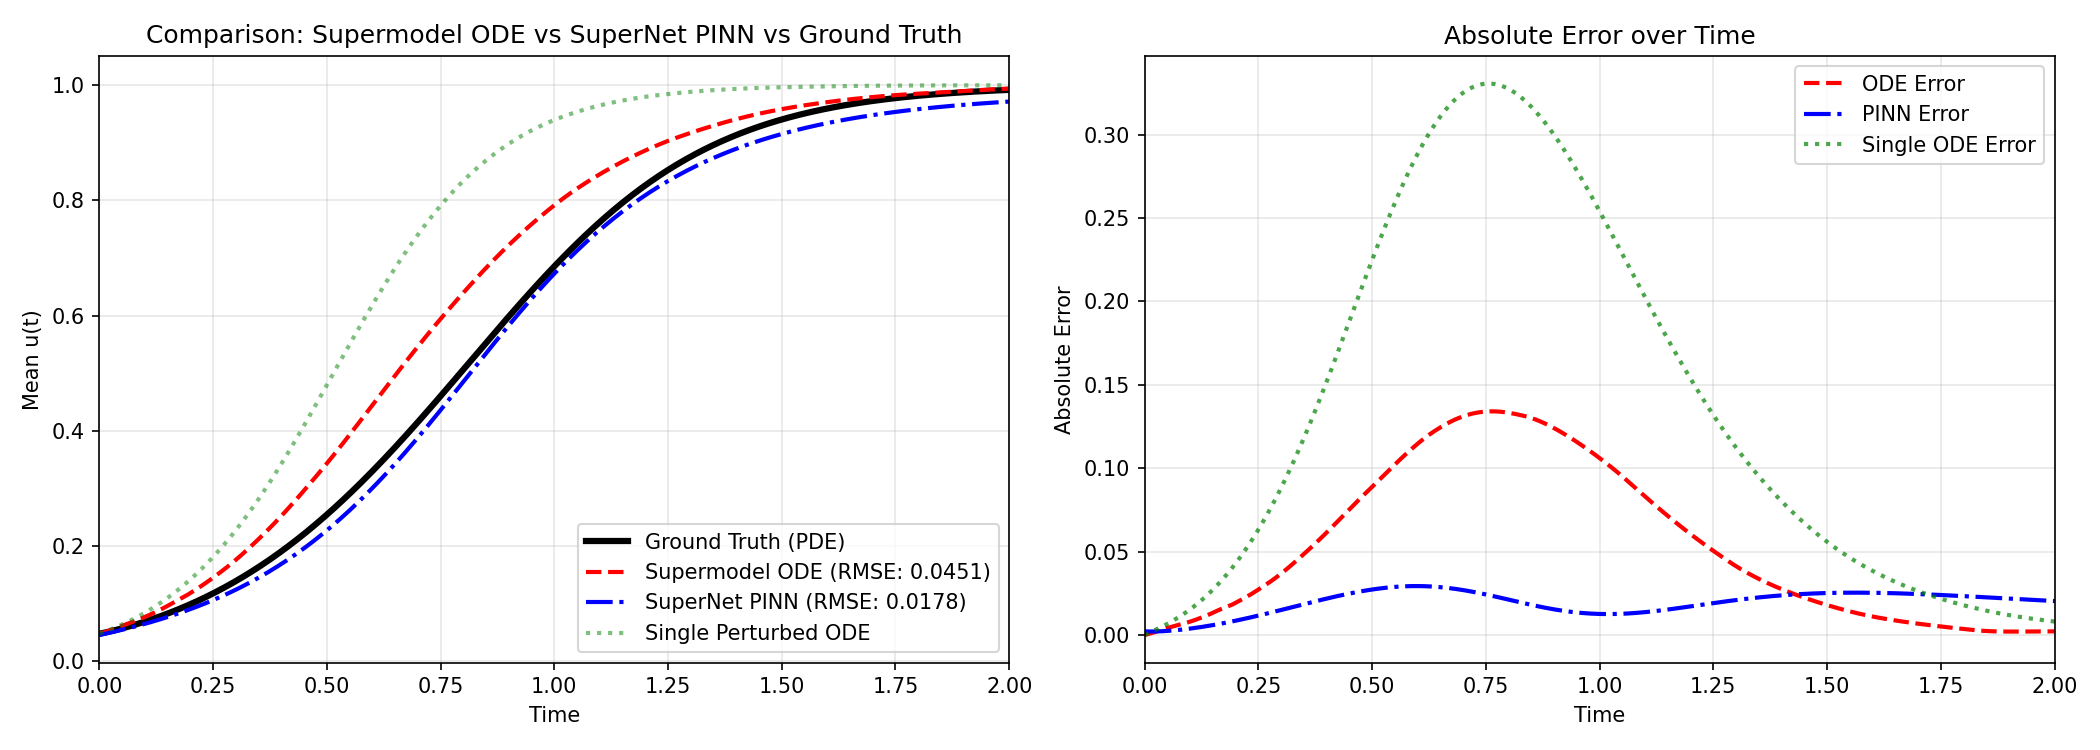
\includegraphics[width=0.49\textwidth]{../zad7/results/supermodel_vs_supernet_improved.png}
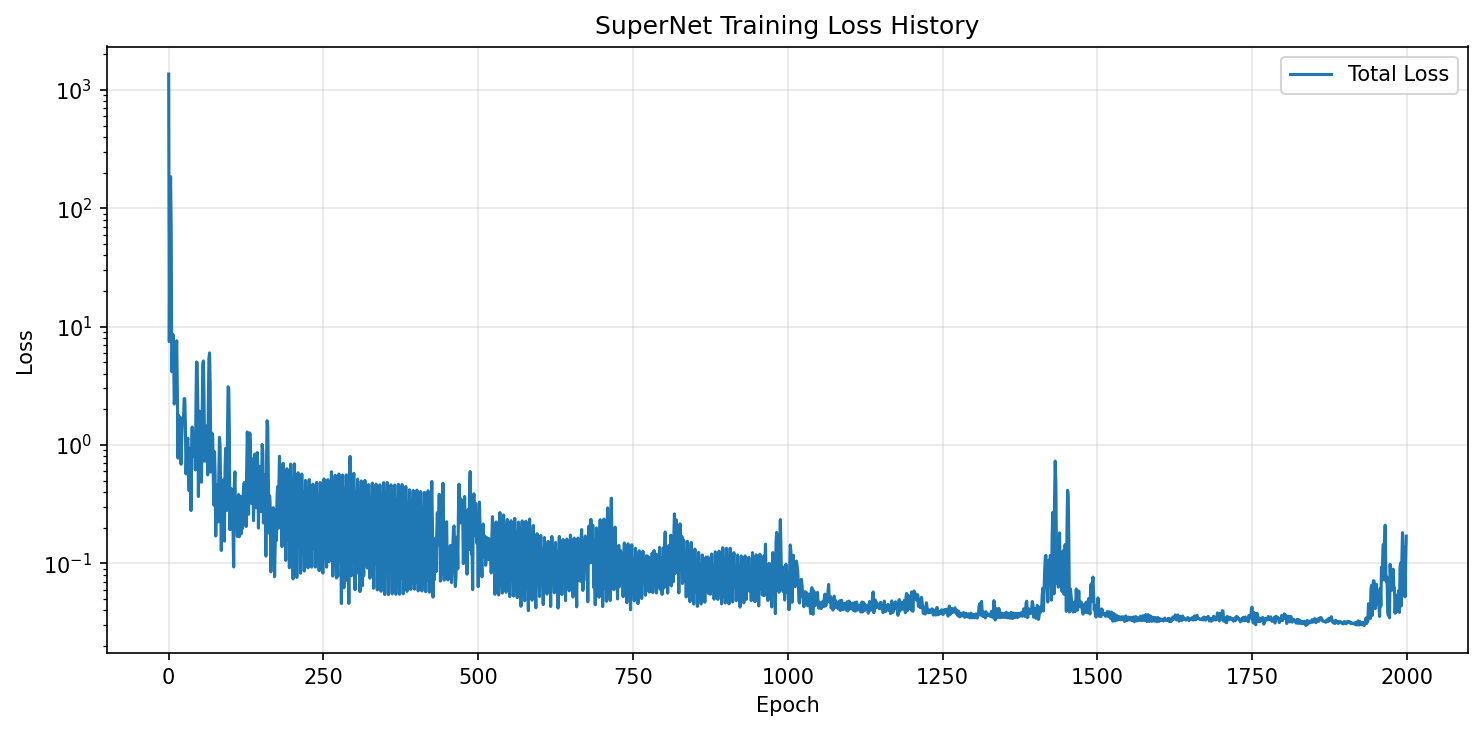
\includegraphics[width=0.49\textwidth]{../zad7/results/supernet_loss_history_improved.png}
\caption{Porównanie jakości predykcji SuperModel vs SuperNet oraz historia utraty dla SuperNet.}
\end{figure}

\section{Szczegółowe zestawienie wyników}
Poniżej przedstawiono zbiorcze zestawienie wybranych metryk i czasów pomiarów, ułatwiające szybkie porównanie rezultatów uzyskanych w różnych zadaniach.

\begin{table}[h]
\centering
\caption{Zestawienie kluczowych wyników projektu}
\begin{tabular}{lrrl}
\toprule
Opis & Wartość 1 & Wartość 2 & Uwagi \\
\midrule
Zadanie 2: explicit (średni czas) & 0.004796 s &  & średnia z 18 prób \\
Zadanie 2: semi-implicit (średni czas) & 0.032856 s &  &  \\
Zadanie 2: crank-nicolson (średni czas) & 0.035034 s &  &  \\
Zadanie 3: ODE (czas inferencji) & 1.2921 ms &  & czas na próbkę \\
Zadanie 3: prosty NN (czas inferencji) & 0.8670 ms &  & czas na próbkę \\
Zadanie 6: PINN (MAE / RMSE) & 0.031193 & 0.058344 & czas tren. 76.58 s \\
Zadanie 7: SuperNet (MAE / RMSE) & 0.017152 & 0.017845 & czas tren. 186.24 s \\
\bottomrule
\end{tabular}
\end{table}

\section{Dyskusja}
Główne obserwacje:
\begin{itemize}
\item Metody jawne (explicit) są bardzo szybkie dla małych rozmiarów siatki, ale w praktyce ich stabilność ogranicza krok czasowy (CFL) — w eksperymentach metoda jawna dawała najkrótszy czas średni.
\item Schematy implicite (CN i półimplicit) są wolniejsze, ale bardziej stabilne i pozwalają na większe kroki czasowe bez utraty stabilności.
\item PINN-y osiągnęły przyzwoitą dokładność (MAE~0.03), co jest konkurencyjne względem klasycznych rozwiązań dla pewnych zadań; ich koszt treningowy jednak jest wyższy niż prostych solverów PDE.
\item SuperNet PINN poprawia średni błąd predykcji w porównaniu do pojedynczego zaburzonego modelu ODE, co pokazuje, że uczenie parametryczne może zwiększać odporność i dokładność.
\end{itemize}

\section{Wnioski}
Projekt pokazał praktyczne różnice między podejściami numerycznymi i uczeniem maszynowym w kontekście równań różniczkowych. Dla zadań wymagających szybkości inferencji warto rozważyć lekkie modele NN, natomiast dla wysokiej dokładności i elastyczności modelowania parametrów rozważne jest zastosowanie PINN / SuperNet.

\subsection*{Ograniczenia i przyszłe prace}
Przeprowadzone eksperymenty mają kilka ograniczeń: zakres parametrów i rozmiarów siatki jest umiarkowany (nx do 200), testy wykonywano na CPU, a optymalizacja hiperparametrów sieci (np. architektura, współczynniki regularizacji) została przeprowadzona tylko w ograniczonym zakresie. Przyszłe prace mogą obejmować: skalowanie eksperymentów na GPU, gruntowne badania wpływu seedów i odchyleń losowych, zastosowanie zaawansowanych technik optymalizacyjnych dla PINN (adaptacyjne wagi strat, większe zbiory danych), oraz porównanie z klasycznymi numerycznymi metodami adaptacyjnymi (np. adaptacyjne siatki czasowo-przestrzenne).

\bibliographystyle{plain}
\nocite{*}
\bibliography{bibliography}

\end{document}
